\documentclass[12pt,a4paper]{article}
\usepackage{graphicx}
\usepackage{hyperref}
\usepackage{geometry}
\usepackage{enumitem}
\usepackage{float}

\geometry{a4paper,left=2.5cm,right=2.5cm,top=2.5cm,bottom=2.5cm}

\title{Lab Report 3: Identifying Running Processes}
\author{GuYi}
\date{\today}

\begin{document}

\maketitle

\section{Lab Objectives}

This lab will use the TCP/UDP Endpoint Viewer tool from Windows Sysinternals Suite to identify processes running on the computer. The specific objectives are as follows:

\begin{itemize}
    \item Download Windows Sysinternals Suite
    \item Launch TCP/UDP Endpoint Viewer
    \item Explore running processes
    \item Explore user-initiated processes
\end{itemize}

\section{Lab Background}

In this lab, we will explore processes. A process is a program or application that is currently executing. We will use Process Explorer from Windows Sysinternals Suite to explore processes, and we will also launch and observe a new process.

\section{Lab Steps}

\subsection{Part 1: Download Windows Sysinternals Suite}

\begin{enumerate}
    \item Navigate to the following link to download Windows Sysinternals Suite:\\
    \url{https://technet.microsoft.com/en-us/sysinternals/bb842062.aspx}
    \item After downloading, right-click on the zip file, select "Extract All...", and extract the files from the folder.
    \item Choose the default name and destination location (Downloads folder), then click "Extract".
    \item Exit the Web browser.
\end{enumerate}

\subsection{Part 2: Launch TCP/UDP Endpoint Viewer}

\begin{enumerate}
    \item Navigate to the SysinternalsSuite folder containing all the extracted files.
    \item Open Tcpview.exe. When prompted, accept the Process Explorer license agreement.
    \item Click "Yes" to allow this application to make changes to your device.
    \item Exit File Explorer and close all currently running applications.
\end{enumerate}

\begin{figure}[H]
    \centering
    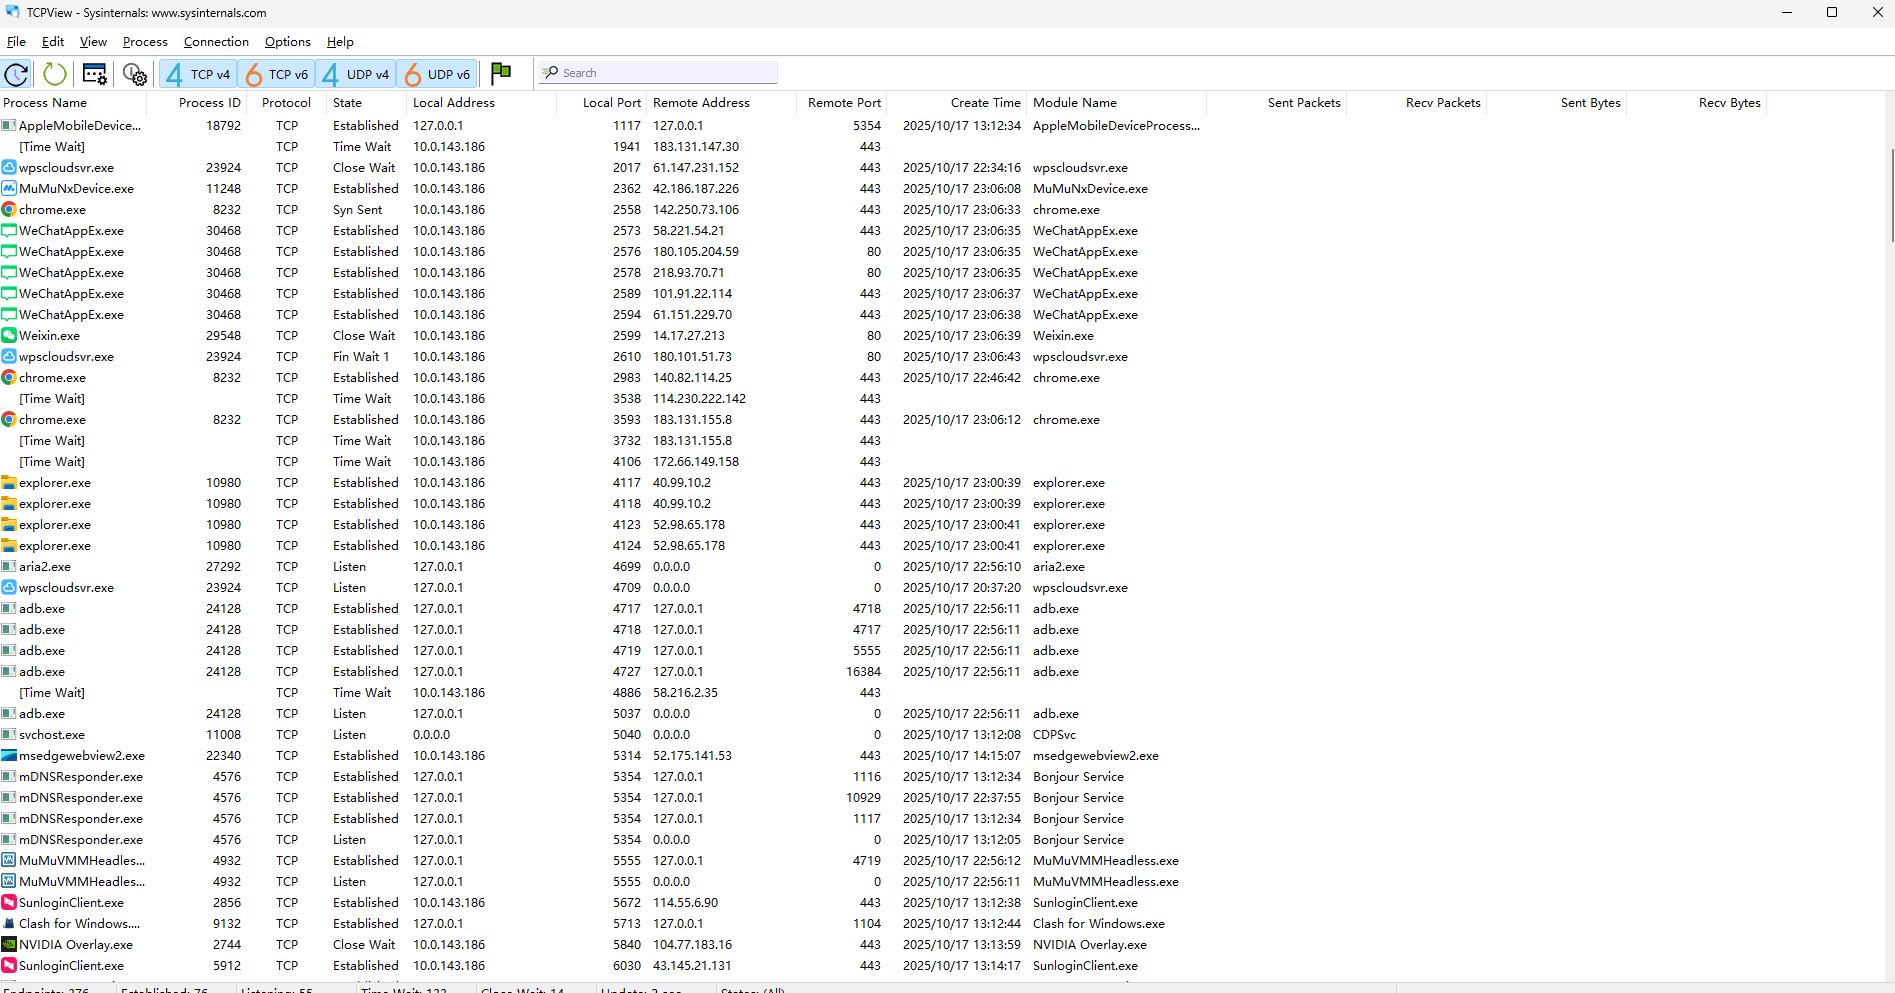
\includegraphics[width=0.8\textwidth]{TcpView.png}
    \caption{TCP/UDP Endpoint Viewer Interface}
    \label{fig:tcpview}
\end{figure}

\subsection{Part 3: Explore Running Processes}

\begin{enumerate}
    \item TCPView lists the currently running processes on your Windows PC. At this point, only Windows processes are running.
    \item Double-click on lsass.exe.
\end{enumerate}

\begin{figure}[H]
    \centering
    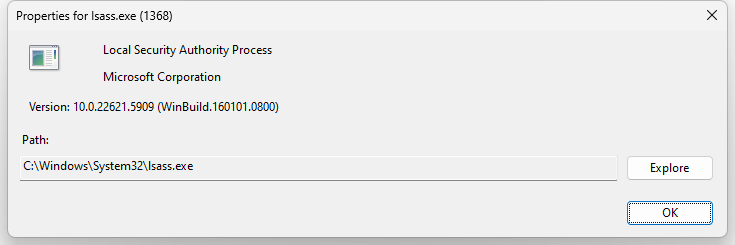
\includegraphics[width=0.8\textwidth]{lssas.png}
    \caption{lsass.exe Process Properties}
    \label{fig:lsass}
\end{figure}

\textbf{Question:}
\begin{itemize}
    \item What is lsass.exe? In which folder is it located?
\end{itemize}

\textbf{Answer:}
lsass.exe is the executable file for the Windows Local Security Authority Subsystem Service. It is responsible for enforcing security policies, verifying user logins to Windows systems, managing password changes, and creating access tokens. As seen in the image, it is located in the C:/Windows/System32 folder. This is a critical Windows system process, and if terminated, the system will become unstable or force a restart.

\begin{enumerate}
    \item[3.] Close the lsass.exe properties window when finished.
    \item[4.] View the properties of other running processes.
\end{enumerate}

\textbf{Note:} Not all processes can have their property information queried.

\subsection{Part 4: Explore User-Initiated Processes}

\begin{enumerate}
    \item Open a Web browser, such as Microsoft Edge.
\end{enumerate}

\begin{figure}[H]
    \centering
    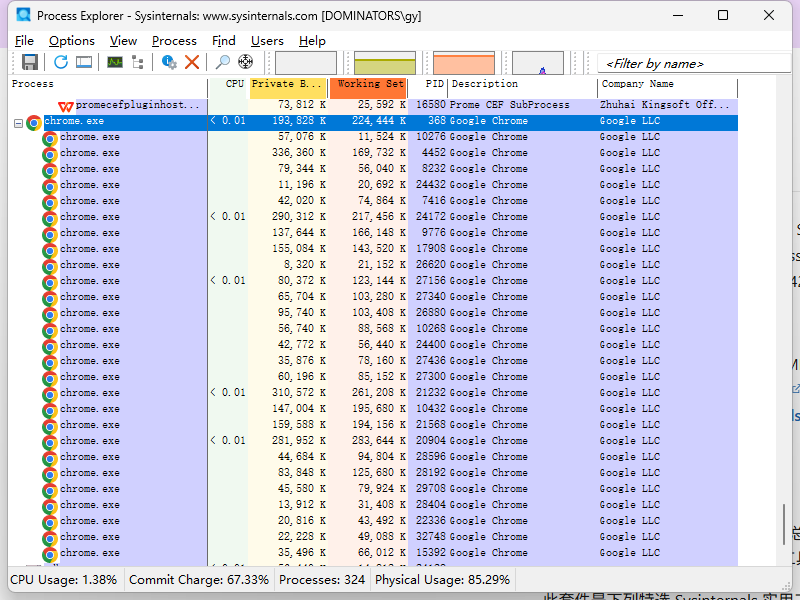
\includegraphics[width=0.8\textwidth]{proecxp.png}
    \caption{Process Explorer Detecting Browser Process}
    \label{fig:procexp}
\end{figure}

\textbf{Question:}
\begin{itemize}
    \item What did you observe in the TCPView window?
\end{itemize}

\textbf{Answer:}
In the TCPView window, when opening a web browser (such as Microsoft Edge), multiple new network connections can be observed being created. These connections show the TCP/UDP connections established between the browser process and various remote servers. The browser process can be seen using different local ports to communicate with remote servers, including DNS queries (for domain name resolution), HTTP/HTTPS connections (for loading web content), and other possible connections (such as WebSocket, content delivery networks, etc.). The status of these connections (such as ESTABLISHED, LISTENING, CLOSE\_WAIT, etc.) is also displayed in TCPView.

\begin{enumerate}
    \item[2.] Close the Web browser.
\end{enumerate}

\textbf{Question:}
\begin{itemize}
    \item What did you observe in the TCPView window?
\end{itemize}

\textbf{Answer:}
After closing the web browser, all connections related to the browser disappear from the TCPView window. This indicates that when an application is closed, its related network connections are also terminated. TCPView briefly displays these closed connections with a color change (usually red) before they completely disappear from the list. The system returns to displaying only the network connection status of basic Windows system processes.

\section{Lab 2: Exploring Processes, Threads, Handles, and Windows Registry}

\subsection{Part 1: Exploring Processes}

\begin{figure}[H]
    \centering
    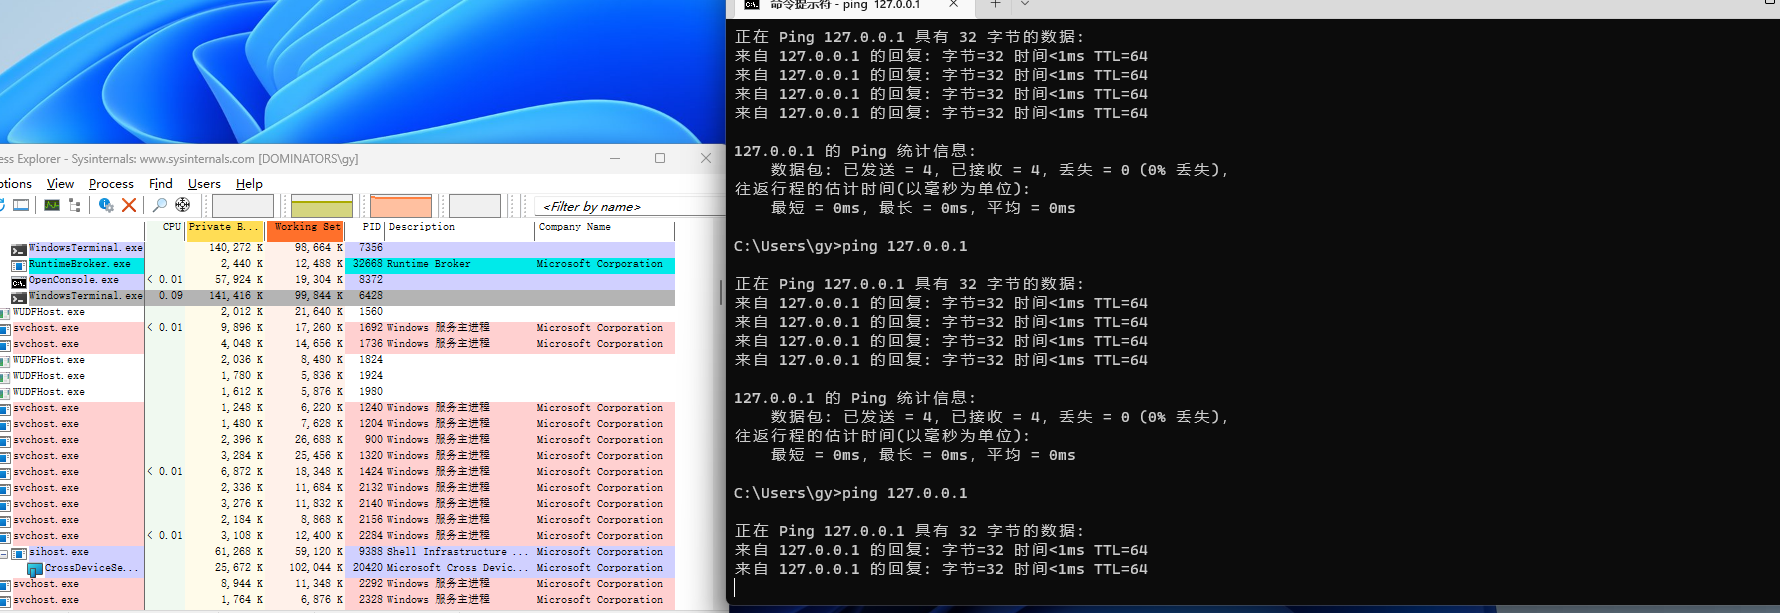
\includegraphics[width=0.8\textwidth]{cmd.png}
    \caption{Process Explorer Detecting Command Prompt Process}
    \label{fig:cmd}
\end{figure}

\textbf{Question:}
\begin{itemize}
    \item What happened to the Web browser window when the process was terminated?
\end{itemize}

\textbf{Answer:}
When terminating the web browser process using Process Explorer, the browser window closes immediately without any warning or save prompts. This is because terminating a process forcibly ends all threads and resources of that process, giving the application no opportunity to execute normal closing procedures (such as saving data or closing connections). This can lead to loss of unsaved data and possibly loss of browsing history or session data in some cases.

\textbf{Question:}
\begin{itemize}
    \item What happened during the ping process?
\end{itemize}

\textbf{Answer:}
During the execution of the ping command, new activity can be observed under the cmd.exe process in Process Explorer. Specifically, small fluctuations in CPU usage can be seen, indicating that the ping command is performing network operations. In the thread view, the thread responsible for executing the ping command can be seen in an active state. Additionally, network-related handles being created and used can be observed, which are used for sending ICMP request packets and receiving response packets. The ping command itself does not create a new child process but executes as a command within the cmd.exe process.

\textbf{Question:}
\begin{itemize}
    \item What happened to the child process conhost.exe when the cmd.exe process was terminated?
\end{itemize}

\textbf{Answer:}
When the cmd.exe process is terminated, its child process conhost.exe (console host process) is also automatically terminated. This is because conhost.exe is a process that provides console window services for cmd.exe, and they have a parent-child relationship. In Windows, when a parent process is terminated, the operating system typically terminates all related child processes. This behavior ensures that no orphaned processes continue to run, preventing resource leaks and system instability.

\subsection{Part 2: Exploring Threads and Handles}

\begin{figure}[H]
    \centering
    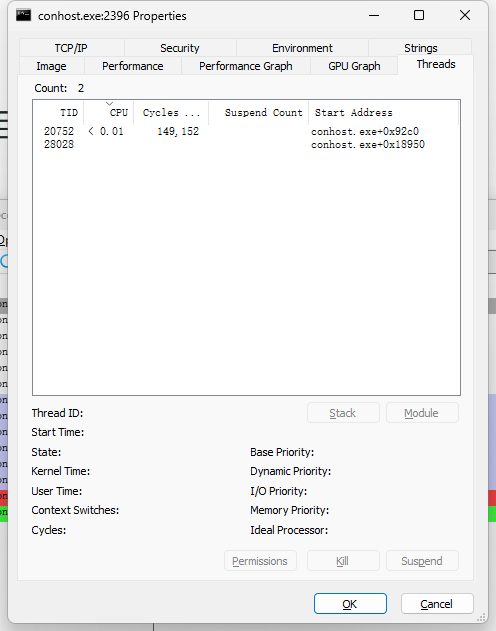
\includegraphics[width=0.8\textwidth]{Thread.png}
    \caption{Process Thread Properties}
    \label{fig:thread}
\end{figure}

\textbf{Question:}
\begin{itemize}
    \item What types of information are available in the thread properties window?
\end{itemize}

\textbf{Answer:}
In the thread properties window, the following types of information can be seen:
\begin{itemize}
    \item Thread ID (TID): Unique identifier for each thread
    \item CPU usage and execution time of the thread
    \item Thread priority and status (such as running, waiting, suspended, etc.)
    \item Thread start address and current execution location
    \item Thread stack information, showing function call hierarchy
    \item Thread context switch count
    \item Module (DLL) to which the thread belongs
    \item Thread creation time
\end{itemize}
This information is very useful for understanding the execution flow within a process and diagnosing performance issues.

\begin{figure}[H]
    \centering
    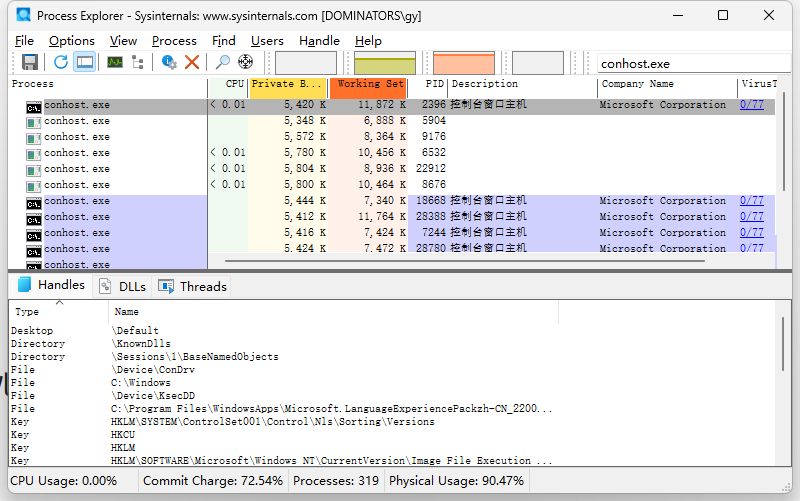
\includegraphics[width=0.8\textwidth]{handles.png}
    \caption{Process Handle Properties}
    \label{fig:handles}
\end{figure}

\textbf{Question:}
\begin{itemize}
    \item What do handles point to?
\end{itemize}

\textbf{Answer:}
In the Process Explorer handle view, handles can be seen pointing to various system resources, including:
\begin{itemize}
    \item Files: Files opened by the process, including executable files, configuration files, data files, etc.
    \item Registry keys: Windows registry entries accessed by the process
    \item Directories: File system directories accessed by the process
    \item Events: Event objects used for inter-process synchronization
    \item Mutexes: Synchronization objects used to control access to shared resources
    \item Semaphores: Synchronization objects used to control resource access counts
    \item Threads: Thread objects created or accessed by the process
    \item Processes: Other processes referenced by the current process
    \item Devices: References to hardware devices or virtual devices
    \item Ports: Communication ports, such as named pipes or network ports
\end{itemize}
These handles are essentially references to operating system resources, through which processes interact with system resources.

\subsection{Part 3: Exploring Windows Registry}

\begin{figure}[H]
    \centering
    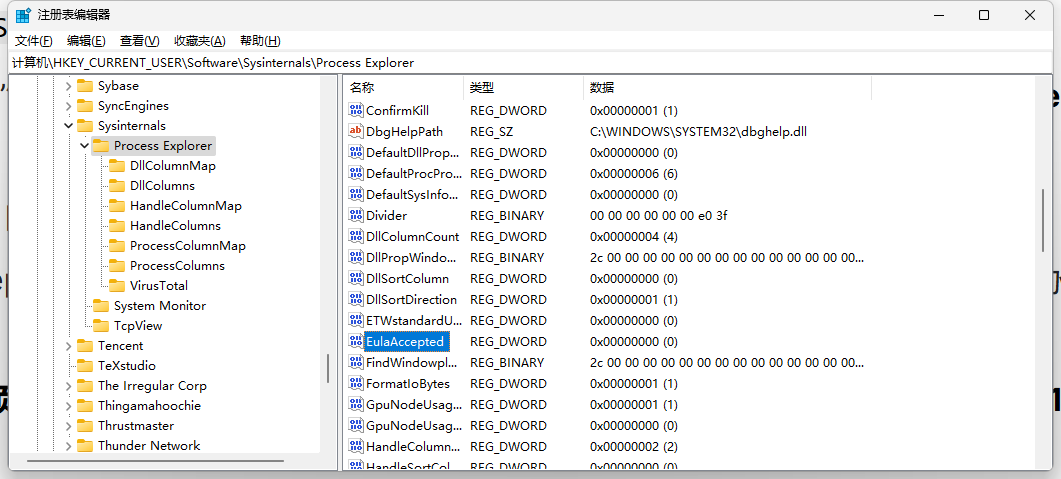
\includegraphics[width=0.8\textwidth]{Eula.png}
    \caption{EULA Settings in Registry}
    \label{fig:eula}
\end{figure}

\textbf{Question:}
\begin{itemize}
    \item What is the value of the EulaAccepted registry key?
\end{itemize}

\textbf{Answer:}
The value of the EulaAccepted registry key is 0x00000001(1), indicating that the user has accepted the End User License Agreement (EULA) for Process Explorer. This value is stored under the path HKEY\_CURRENT\_USER\\Software\\Sysinternals\\Process Explorer. When the value is 1, it indicates that the EULA has been accepted; when the value is 0, it indicates that the EULA has not yet been accepted.

\begin{figure}[H]
    \centering
    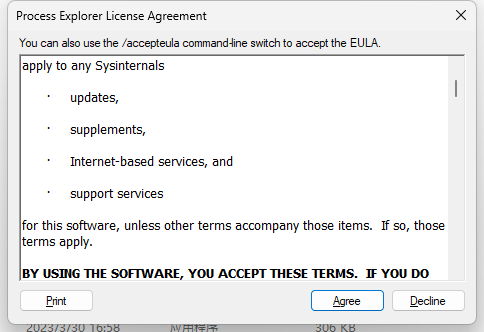
\includegraphics[width=0.8\textwidth]{Eula_0_result.png}
    \caption{Result After Changing EulaAccepted Value to 0}
    \label{fig:eula_result}
\end{figure}

\textbf{Question:}
\begin{itemize}
    \item What did you see when you opened Process Explorer after changing the EulaAccepted value from 1 to 0?
\end{itemize}

\textbf{Answer:}
After changing the EulaAccepted value from 1 to 0 and opening Process Explorer, the software displays the End User License Agreement (EULA) dialog box again, requiring the user to re-accept the license terms. This indicates that Process Explorer checks this value in the registry each time it starts to determine whether to display the EULA. If the user accepts the EULA, the value is reset to 1; if the user refuses to accept, the application will not start. This is a mechanism for the software to ensure that users understand and agree to the terms of use.

\section{Lab Conclusion}

Through this lab, we have successfully used tools from Windows Sysinternals Suite to explore and analyze processes, threads, handles, and the registry in Windows systems. We have learned:

\begin{itemize}
    \item How to use TCP/UDP Endpoint Viewer and Process Explorer to monitor system processes
    \item The hierarchical structure of processes and parent-child relationships
    \item The characteristics and properties of threads as execution units within processes
    \item How handles serve as references for processes to interact with system resources
    \item How the Windows registry stores application configuration information
    \item How to change application behavior by modifying registry values
\end{itemize}

This knowledge is very important for system administration, security analysis, and software development, helping us better understand the internal working mechanisms of the Windows operating system.

\end{document}